\documentclass[12pt,a4paper]{article}
\usepackage[utf8]{inputenc}
\usepackage[english]{babel}
%\usepackage{minted}
\usepackage{listings}
\usepackage{xcolor}
\usepackage{graphicx}

%For syntax highlighting
\definecolor{codegreen}{rgb}{0,0.6,0}
\definecolor{codegray}{rgb}{0.5,0.5,0.5}
\definecolor{codepurple}{rgb}{0.58,0,0.82}
\definecolor{backcolour}{rgb}{1,1,1}

%%Sets different parameters
\lstdefinestyle{mystyle}{
	backgroundcolor=\color{backcolour},   
    commentstyle=\color{codegreen},
    keywordstyle=\color{magenta},
    numberstyle=\tiny\color{codegray},
    stringstyle=\color{codepurple},
    basicstyle=\ttfamily\footnotesize,
    breakatwhitespace=false,         
    breaklines=true,                 
    captionpos=b,                    
    keepspaces=true,                 
    numbers=left,                    
    numbersep=5pt,                  
    showspaces=false,                
    showstringspaces=false,
    showtabs=false,                  
    tabsize=4
}
\lstset{style=mystyle}

\begin{document}
\section*{\centering{\textbf{8 bit Arithmetic Operations}}}

\begin{table}[h]
\resizebox{\textwidth}{!}{
    \small{
    \begin{tabular}{l r}
        Exp. No.: 1  & Name: Shivanirudh S G\\
        Date: 30 August 2020 & Reg. No.: 185001146\\
    \end{tabular}
    }
}
\end{table}

\bigskip
\hrule
\begin{flushleft}
\subsection*{\textbf{Aim:}} 
To perform arithmetic operations on two 8 bit numbers.

\subsection*{\textbf{Procedure:}}
\begin{itemize}
    \item Mount masm folder to a drive on DOSBOX.
    \item Go to mounted drive.
    \item Save 8086 program with the extension \textbf{``.asm"} in the same folder using the command \textbf{``edit"}.
    \item Assemble the \textbf{.asm} file using the command \textbf{``masm filename.asm"}.
    \item Link the assmebled \textbf{.obj} file using the command \textbf{``link filename.obj"}.
    \item Debug the executable file \textbf{.exe} with the \textbf{``debug filename.exe"} command.
    \begin{itemize}
        \item The unassembled code can be viewed by the command \textbf{``u"}.
        \item Use the command \textbf{``d segment:offset"} to view the contents of memory locations from the specified segment:offset address.
        \item Use command \textbf{``e segment:offset"} to change the values in memory.
        \item Execute the program using command \textbf{``g"}.
        \item The command \textbf{``q"} exits from the debug session.
    \end{itemize}
\end{itemize}
\subsection*{\textbf{Algorithm:}}
\begin{enumerate}
    \item Begin.
    \item Declare data and code segments.
    \item Declare variables for operands, and results in the data segment.
    \item Start code segment.
    \item Set an offset if preferred.
    \item Load contents of the data segment into the DS register through the AX register.
    \item Load contents of the operand(s) on to AL and/or BL register(s).
    \item Perform required operation, add, sub, mul or div, on the operands.
    \item If a carry/overflow occurs, store it.
    \item Store results in respective registers.
    \item Request Interrupt to terminate.
    \item End code segment.
    \item End. 
\end{enumerate}
\hrule
\newpage
\subsection*{\textbf{\underline{8 Bit Addition}}}

\subsubsection*{\textbf{Program:}}

\begin{table}[htb]
\centering\small
\resizebox{\columnwidth}{!}{
\begin{tabular}{|l|l|} 
\hline
\textbf{Program}                                                 & \textbf{Comments}                             \\ 
\hline
assume cs:code,ds:data                                           & Declare code and data segments                \\ 
\hline
data segment                                                     & Declare operands in data segment              \\ 
\hline
opr1 db 11h                                                      & Set opr1 to hex value 11                      \\ 
\hline
opr2 db 99h                                                      & Set opr2 to hex value 99                      \\ 
\hline
result db 00H                                                    & Set result to hex value 00                    \\ 
\hline
carry db 00H                                                     & Set carry to hex value 00                     \\ 
\hline
data ends                                                        & End of data segment                           \\ 
\hline
code segment                                                     &                                               \\ 
\hline
org 0100h                                                        &                                               \\ 
\hline
start:~ mov ax,data                                              & Move data segment contents to AX register     \\ 
\hline
mov ds,ax                                                        & Move data in AX register to DS register       \\ 
\hline
mov ah,opr1                                                      & Move contents of opr1 to AH register          \\ 
\hline
mov bh,opr2                                                      & Move contents of opr2 to BH register          \\ 
\hline
mov ch,00h                                                       & Move hex value 00 to CH register              \\ 
\hline
add ah,bh                                                        & AH = AH + BH                                  \\ 
\hline
jnc here                                                         & Jump to the label here, if there is no carry  \\ 
\hline
inc ch                                                           & Increment value of CH if there is a carry     \\ 
\hline
here:~ mov result,ah                                             & Move contents of AH register to result        \\ 
\hline
mov carry,ch                                                     & Move contents of CH register to carry         \\ 
\hline
mov ah,4ch                                                       &                                               \\ 
\hline
int 21h                                                          & Request interrupt routine                     \\ 
\hline
code ends                                                        &                                               \\ 
\hline
end start                                                        &                                               \\
\hline
\end{tabular}
}
\end{table}

%\newpage
\subsubsection*{\textbf{Input and Output:}}
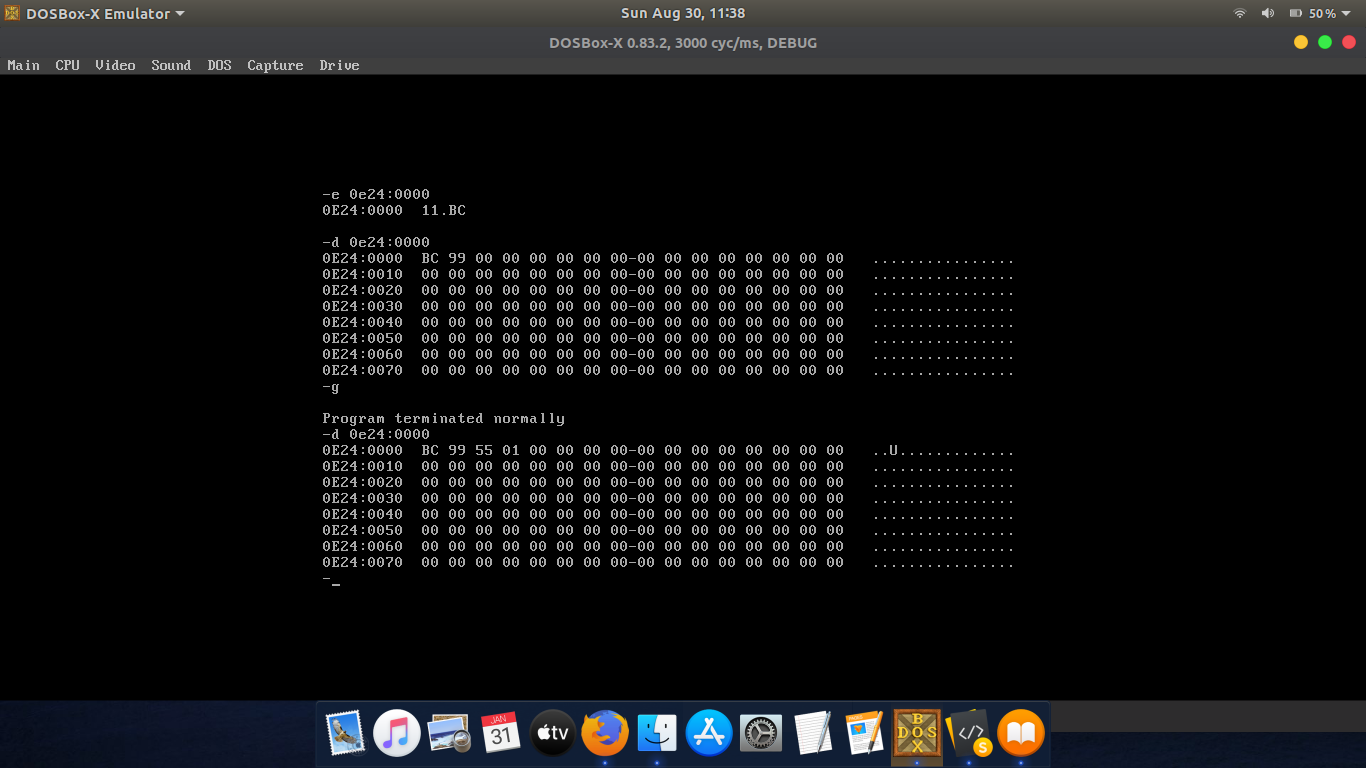
\includegraphics[trim = 100mm 60mm 100mm 80mm, clip, width = \textwidth]{Addition.png}

%----------------------------------------------------------------------------------------------------------------------------------------
\newpage
\subsection*{\textbf{\underline{8 Bit Subtraction}}}

\subsubsection*{\textbf{Program:}}
\begin{table}[htb]
\centering\small
\resizebox{\columnwidth}{!}{
\begin{tabular}{|l|l|} 
\hline
\textbf{Program}                                                 & \textbf{Comments}                             \\ 
\hline
assume cs:code,ds:data                                           & Declare code and data segments                \\ 
\hline
data segment                                                     & Declare operands in data segment              \\ 
\hline
opr1 db 11h                                                      & Set opr1 to hex value 11                      \\ 
\hline
opr2 db 99h                                                      & Set opr2 to hex value 99                      \\ 
\hline
result db 00H                                                    & Set result to hex value 00                    \\ 
\hline
carry db 00H                                                     & Set carry to hex value 00                     \\ 
\hline
data ends                                                        & End of data segment                           \\ 
\hline
code segment                                                     &                                               \\ 
\hline
org 0100h                                                        &                                               \\ 
\hline
start:~ mov ax,data                                              & Move data segment contents to AX register     \\ 
\hline
mov ds,ax                                                        & Move data in AX register to DS register       \\ 
\hline
mov ah,opr1                                                      & Move contents of opr1 to AH register          \\ 
\hline
mov bh,opr2                                                      & Move contents of opr2 to BH register          \\ 
\hline
mov ch,00h                                                       & Move hex value 00 to CH register              \\ 
\hline
sub ah,bh                                                        & AH = AH - BH                                  \\ 
\hline
jnc here                                                         & Jump to the label here, if there is no carry  \\ 
\hline
inc ch                                                           & Increment value of CH if there is a carry     \\ 
\hline
neg ah                                                           & Negate the contents of the AH register        \\
\hline
here:~ mov result,ah                                             & Move contents of AH register to result        \\ 
\hline
mov carry,ch                                                     & Move contents of CH register to carry         \\ 
\hline
mov ah,4ch                                                       &                                               \\ 
\hline
int 21h                                                          & Request interrupt routine                     \\ 
\hline
code ends                                                        &                                               \\ 
\hline
end start                                                        &                                               \\
\hline
\end{tabular}
}
\end{table}

%\newpage
\subsubsection*{\textbf{Input and Output:}}
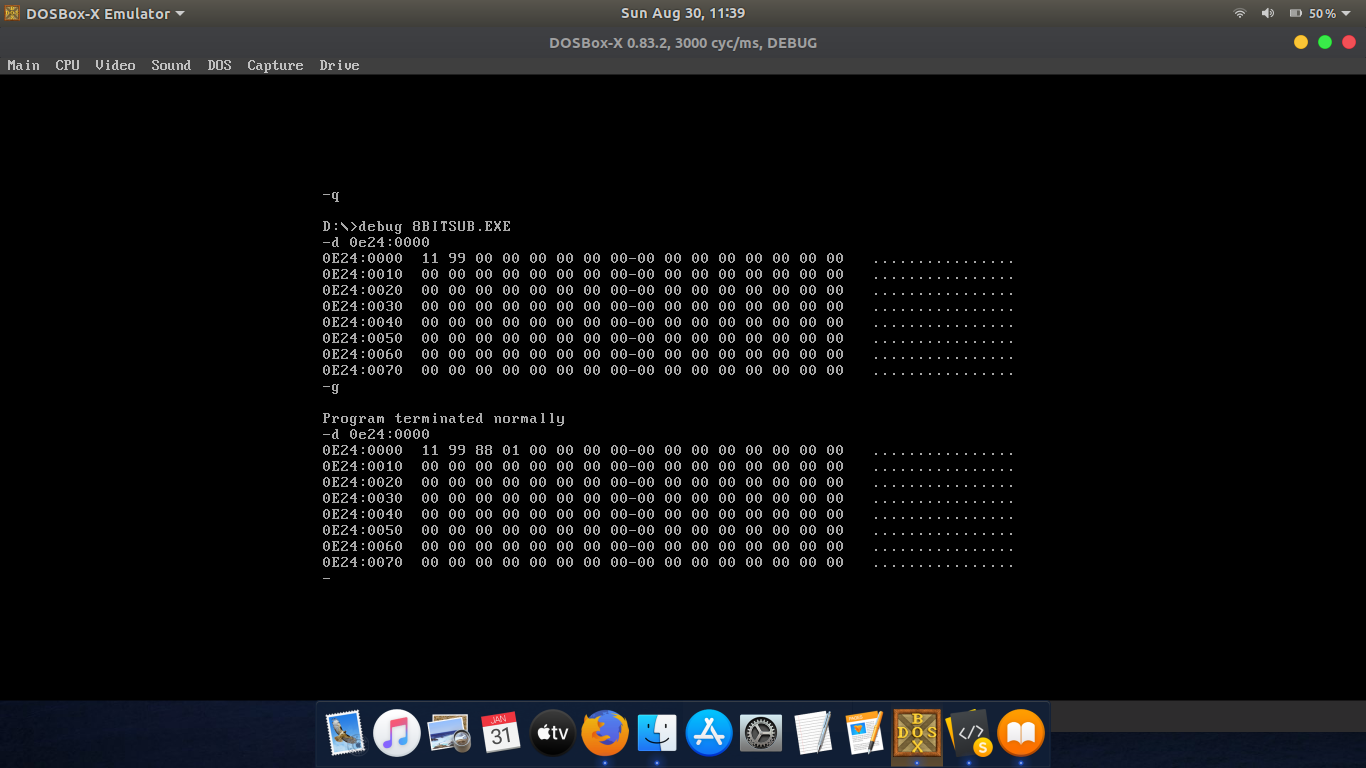
\includegraphics[trim = 100mm 60mm 100mm 80mm, clip, width = \textwidth]{Subtraction.png}

%----------------------------------------------------------------------------------------------------------------------------------------
\newpage
\subsection*{\textbf{\underline{8 Bit Multiplication}}}

\subsubsection*{\textbf{Program:}}
\begin{table}[htb]
\centering\small
\resizebox{\columnwidth}{!}{
\begin{tabular}{|l|l|} 
\hline
\textbf{Program}                                                 & \textbf{Comments}                             \\ 
\hline
assume cs:code,ds:data                                           & Declare code and data segments                \\ 
\hline
data segment                                                     & Declare operands in data segment              \\ 
\hline
opr1 db 11h                                                      & Set opr1 to hex value 11                      \\ 
\hline
opr2 db 99h                                                      & Set opr2 to hex value 99                      \\ 
\hline
resulth db 00H                                                   & Set resulth to hex value 00                   \\ 
\hline
resultl db 00H                                                   & Set resultl to hex value 00                   \\ 
\hline
data ends                                                        & End of data segment                           \\ 
\hline
code segment                                                     &                                               \\ 
\hline
org 0100h                                                        &                                               \\ 
\hline
start:~ mov ax,data                                              & Move data segment contents to AX register     \\ 
\hline
mov ds,ax                                                        & Move data in AX register to DS register       \\ 
\hline
mov al,opr1                                                      & Move contents of opr1 to AL register          \\ 
\hline
mov ah, 00H                                                      & Move hex value 00 to AH register              \\
\hline
mov bh,opr2                                                      & Move contents of opr2 to BH register          \\ 
\hline
mul bh                                                           & AX = AL * BH                                  \\ 
\hline
here:~ mov resulth,ah                                            & Move contents of AH register to resulth       \\ 
\hline
mov resultl,al                                                   & Move contents of AL register to resultl       \\ 
\hline
mov ah,4ch                                                       &                                               \\ 
\hline
int 21h                                                          & Request interrupt routine                     \\ 
\hline
code ends                                                        &                                               \\ 
\hline
end start                                                        &                                               \\
\hline
\end{tabular}
}
\end{table}

%\newpage
\subsubsection*{\textbf{Input and Output:}}
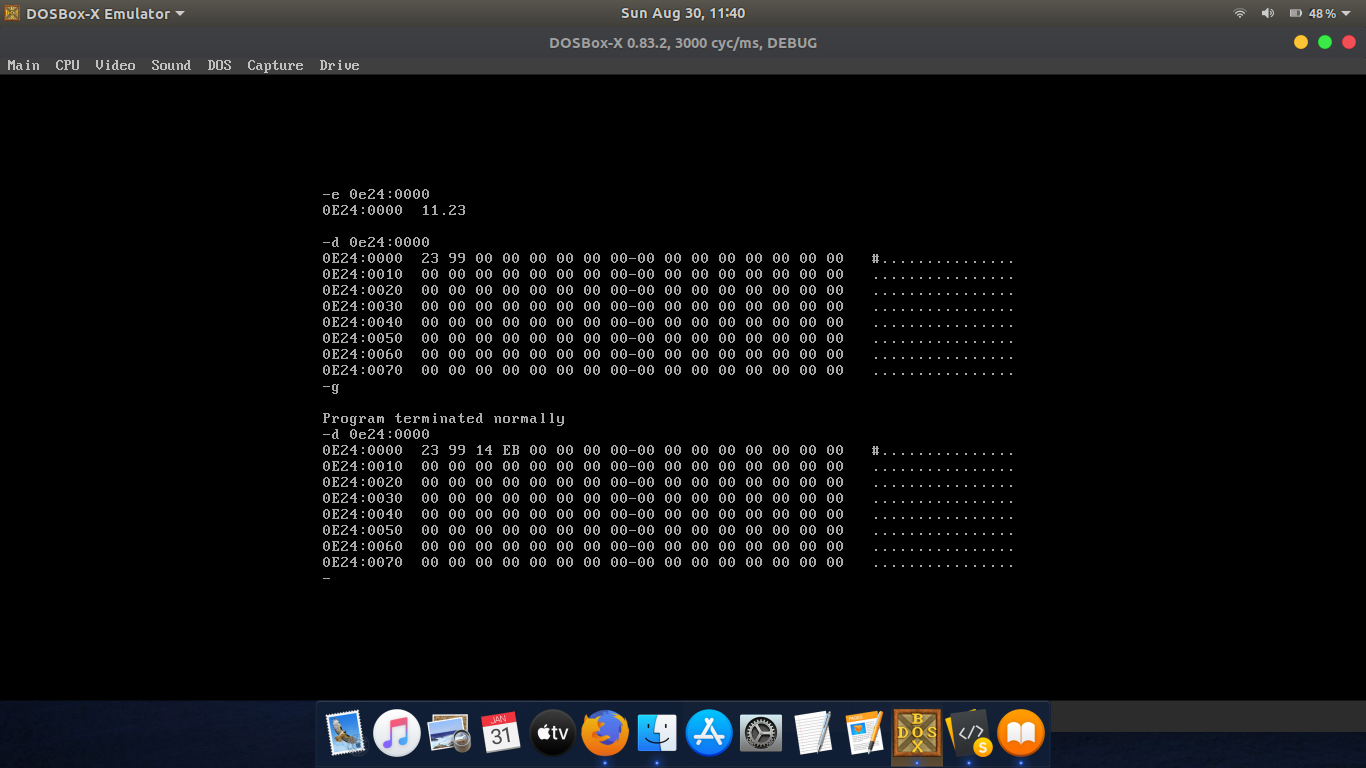
\includegraphics[trim = 100mm 60mm 100mm 80mm, clip, width = \textwidth]{Multiplication.png}

%----------------------------------------------------------------------------------------------------------------------------------------
\newpage
\subsection*{\textbf{\underline{8 Bit Division}}}

\subsubsection*{\textbf{Program:}}
\begin{table}[h]
\centering\small
\resizebox{\columnwidth}{!}{
\begin{tabular}{|l|l|} 
\hline
\textbf{Program}                                                 & \textbf{Comments}                             \\ 
\hline
assume cs:code,ds:data                                           & Declare code and data segments                \\ 
\hline
data segment                                                     & Declare operands in data segment              \\ 
\hline
opr1 db 11h                                                      & Set opr1 to hex value 11                      \\ 
\hline
opr2 db 99h                                                      & Set opr2 to hex value 99                      \\ 
\hline
resultq db 00H                                                   & Set resultq to hex value 00                   \\ 
\hline
resultr db 00H                                                   & Set resultr to hex value 00                   \\ 
\hline
data ends                                                        & End of data segment                           \\ 
\hline
code segment                                                     &                                               \\ 
\hline
org 0100h                                                        &                                               \\ 
\hline
start:~ mov ax,data                                              & Move data segment contents to AX register     \\ 
\hline
mov ds,ax                                                        & Move data in AX register to DS register       \\ 
\hline
mov al,opr1                                                      & Move contents of opr1 to AL register          \\ 
\hline
mov ah, 00H                                                      & Move hex value 00 to AH register              \\
\hline
mov bh,opr2                                                      & Move contents of opr2 to BH register          \\ 
\hline
div bh                                                           & AX = AL / BH                                  \\ 
\hline
here:~ mov resultq,ah                                            & Move contents of AH register to resulth       \\ 
\hline
mov resultr,al                                                   & Move contents of AL register to resultl       \\ 
\hline
mov ah,4ch                                                       &                                               \\ 
\hline
int 21h                                                          & Request interrupt routine                     \\ 
\hline
code ends                                                        &                                               \\ 
\hline
end start                                                        &                                               \\
\hline
\end{tabular}
}
\end{table}

%\newpage
\subsubsection*{\textbf{Input and Output:}}
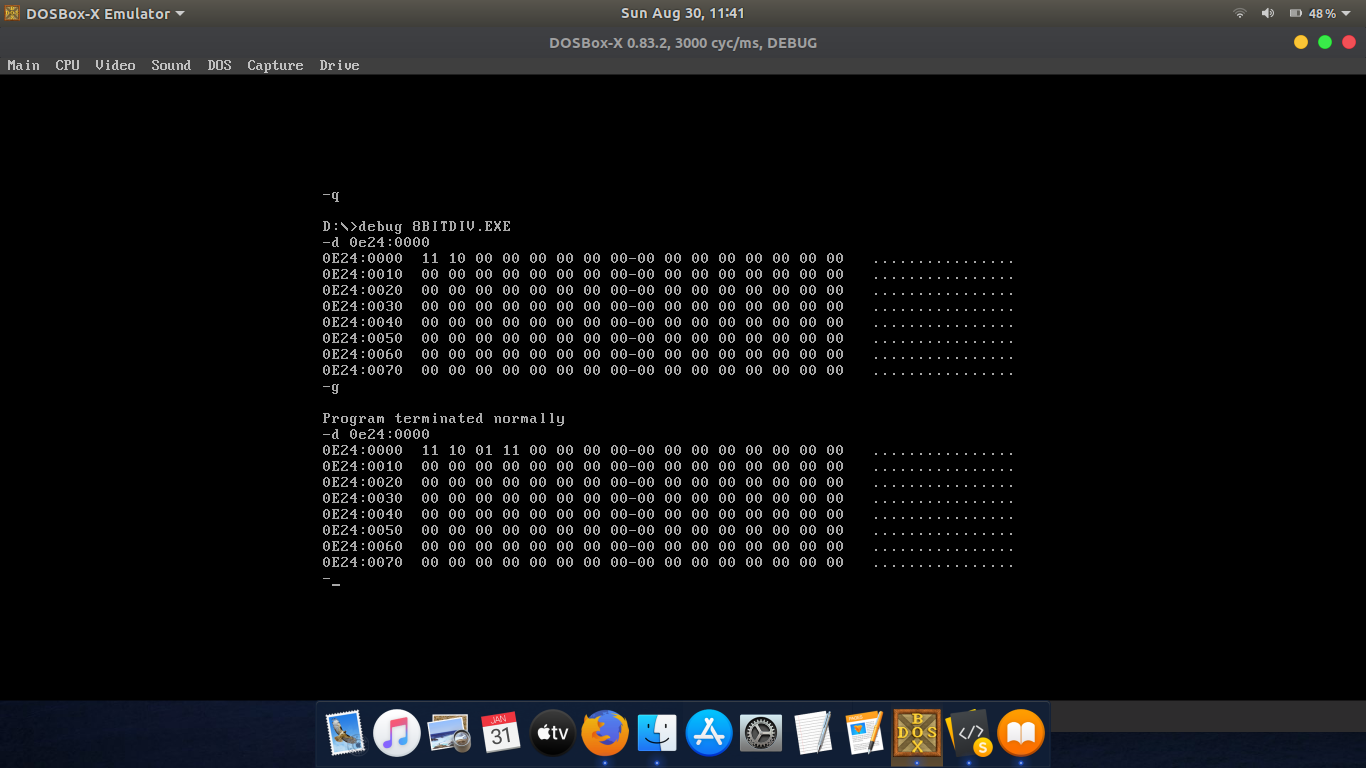
\includegraphics[trim = 100mm 60mm 100mm 80mm, clip, width = \textwidth]{Division.png}

\hrule
\subsection*{\textbf{Result:}}
The 8086 programs were written to perform 8-bit arithmetic operations, and the results observed.
\end{flushleft}
\end{document}